%I have quickly decided to collect the kernel by collecting classes, copying them (without recompiling them) in a new SystemDictionary, and then to fix all the references. 
%
%The point was which classes have to be collected. For my first attempts, I just tried to collect all classes Object depends on. I knew it will be huge, but at least I will not have dependencies to object not in my Hazel world.
%Unfortunately it was almost half of the system, and it is not effective for a minimal kernel.
%
%So I changed my point of view and decided to provide a list of classes to the builder with only the classes I want. It brings new problems, the most important one was how to fix dependencies to the old world, but moreover, it didn't answer to the question which classes should I choose.
%
%To be able to choose, I've analyze dependencies between packages. At least a package is named Kernel, so I started from this package then recursively analyze dependencies. It was quite difficult because I doesn't know the whole system very well and for each dependence, I had to choose. Due to that, I've learned a lot about the system and it structure.
%
%So at this point, I was able to select the classes then to copy them into the Hazel SystemDictionary, but references still point to \gls{Pharo} classes (see Figure~\ref{ClassesCopy}).

\goal
The goal of this part is to create an alternative SystemDictionary (a SystemDictionary is a namespace holding all the classes of the system) starting from the \gls{Pharo} one and to collect classes which are needed to build the kernel. 

\problems
\begin{itemize}
	\item Which classes need to be collected ?
	\item How do we fill up the new SystemDictionary with those classes ?
\end{itemize}

\solutions
\begin{itemize}
	\item A first naive approach is to collect every classes \ct{Object} depends on in order to have an autonomous system. But due to bad dependencies in the system, the kernel collected this way contains half of the \gls{Pharo} classes. This is clearly not working. Therefore we have decided to have another approach. The second and final approach is to provide to the builder the list of classes the user wants in the new kernel plus some classes absolutely needed by the system\footnote{as \ct{Object}, \ct{ProtoObject} or \ct{MethodContext} for example}. The problem is that we had to determine which classes are the absolutely needed ones. In order to answer this question, a tool to analyze classes dependencies has been written and recursively used starting from the Kernel package until we had a quite autonomous kernel composed of around 200 classes\footnote{\gls{Pharo} contains around 1800 classes}. This tool also flags bad dependencies, but this part will be exposed in the next chapter (page~\pageref{KernelIsolation}). 


	\item MicroSqueak's solution to fill up the new \ct{SystemDictionary} is to recompile needed classes with a prefix and then to collect them. It's quite efficient when you have 20 classes to copy, but here we have the constraints that we do not know by advance what we will copy and then we want to be as fast as possible. 
\end{itemize}	
	
The solution we adopted is to create a new instance of \ct{SystemDictionary} and to directly copy classes into it without recompiling them. The classes are still pointing to their original namespace as shown by Figure~\ref{ClassesCopy}.
	
\begin{figure}[h]
	\centering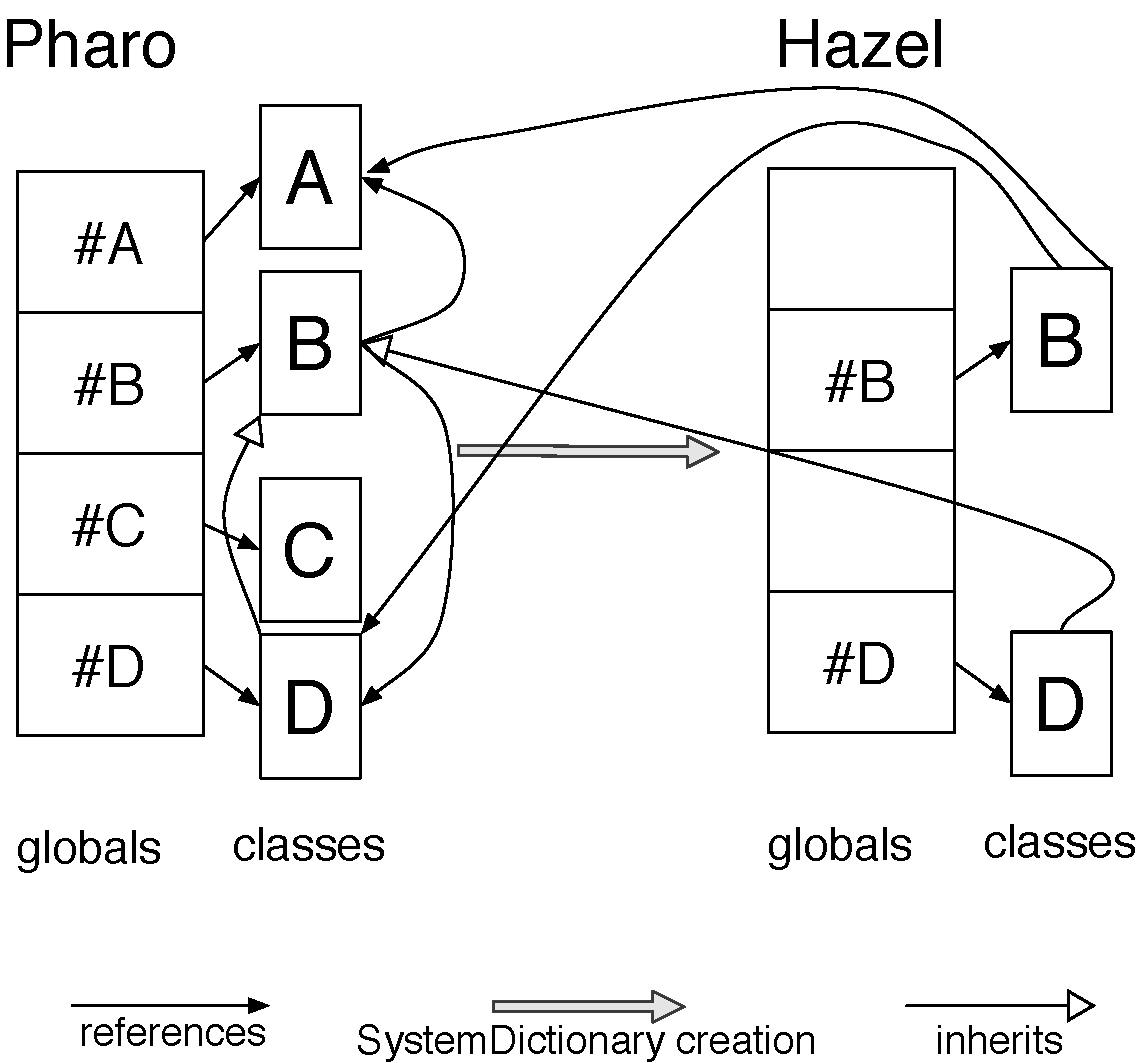
\includegraphics[width = 8cm]{figures/CopyWithInh}
	\caption{Step 1 - Copy the classes \ct{B} and \ct{D} into the new SystemDictionary}
	\label{ClassesCopy}
\end{figure}
	
The second step is to make sure that the class and metaclass hierarchy is maintained in both the environments and that the \ct{methodDictionary}\footnote{a \emph{methodDictionary} is a dictionary implemented in each class and containing all the methods of the class} is also copied. To be sure to reconstruct the hierarchy, the copy method recursively rebuild class, metaclass and superclass hierarchy (see Figure~\ref{ClassMetaClassHierarchy}).

\begin{figure}[h]
	\centering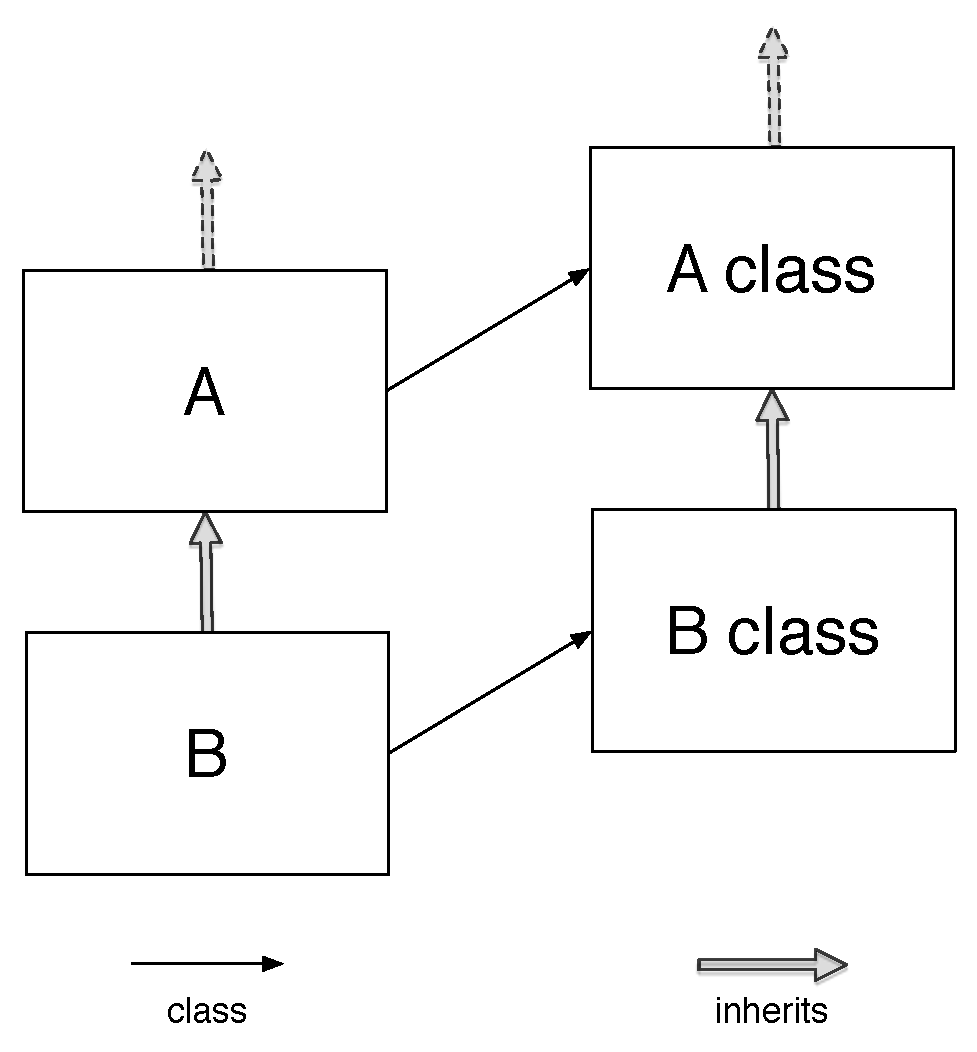
\includegraphics[width = 8cm]{figures/ClassMetaClassHierarchy}
	\caption{Class and MetaClass Hierarchy}
	\label{ClassMetaClassHierarchy}
\end{figure}

	
Here is the pseudo code in Smalltalk that add a class in the Hazel SystemDictionary and check the hierarchy:
	
	\begin{code}{}
		HazelKernelBuilder>>\#addAClassInDictionary: class
		"Add a copy of the class in the Hazel SystemDictionary then answer the copy"

		\tab| hazel copy className |
		\tab className := class name asSymbol.
	
		\tab"Check if the class is already in the dictionary"
		\tab(self list includesKey: class name) 
		\tab\tab	ifFalse: [^ nil].
	
		\tab hazel := Smalltalk at: #HazelSmalltalk.
		\tab(hazel globals includesKey: className) 
		\tab\tab	ifTrue: [^hazel at: className].

		\tab"If not, add a copy in the dictionary"
		\tab copy := self copyClass: class.
		\tab self registerClass: copy.

		\tab"then check the superclass"
		\tab copy superclass ifNotNilDo: [:superclass || superCopy | 
		\tab\tab	"add the superclass"
		\tab\tab	superCopy := self addAClassInDictionary: superclass.
		\tab\tab	"change the superclass"
		\tab\tab	copy superclass: superCopy.
		\tab\tab	"then change the metaclass's superclass"
		\tab\tab	copy class superclass: (superCopy class)].
	
		\tab"Check all literals of all methods"
		\tab self checkMethods: copy.
	
		\tab"Check all class var"
		\tab self checkClassVar: copy.
	
		\tab ^ copy
	\end{code}
	The last instructions will be commented in the next section.
	
	\paragraph{}The only wrong inheritance which remains is that \ct{ProtoObject} in the Hazel world inherits from \ct{nil} which is still in the \gls{Pharo} world. But this will be fixed when we will change \ct{nil} (see paragraph~\ref{NilChange} page~\pageref{NilChange}).


\inanutshell We are now able to copy wanted classes and needed classes into a new \ct{SystemDictionary}, with a good hierarchy, but Hazel classes keep references to \gls{Pharo} ones (see Figure~\ref{ClassesCopy}). 


\newpage